\documentclass{article}
\usepackage[utf8]{inputenc}
\usepackage[margin = 1.1in, headheight = 0.9in, footskip = 0.75 in]{geometry}
\usepackage{fancyhdr}
\usepackage{lastpage}
\usepackage{amsmath}
\usepackage{amssymb}
\usepackage{xparse}
\usepackage{graphicx}
\usepackage{enumerate}
\usepackage{mathtools}
\usepackage{amsthm}
\usepackage{tikz-cd}
\usepackage{tikz}
\usepackage{pgfplots}
\usepackage{bbm}
\usepackage[shortlabels]{enumitem}
\usepackage{algorithm}
\usepackage{algpseudocode}
\usepackage{booktabs}
\usepackage{hyperref}
\hypersetup{
    colorlinks=true,
    linkcolor=black,
    filecolor=magenta,      
    urlcolor=red
    }

\urlstyle{same}
\newcommand{\RNum}[1]{\uppercase\expandafter{\romannumeral #1\relax}}
\newcommand\ddfrac[2]{\frac{\displaystyle #1}{\displaystyle #2}}
\usepackage{xpatch}
\setlength{\parindent}{3em}
\setlength{\parskip}{0.5em}
%===================================================================================================
\pagestyle{fancyplain}
\renewcommand{\headrulewidth}{0pt}
\renewcommand{\footrulewidth}{0pt}
\fancyhf{}\par 
\lhead{\hspace{0cm}\\\hspace{0cm}\\Zmh6339\\AI \& Machine Learning, CS-UH 3260\\Professor Keith Ross}
\rhead{Ziad Hassan\\January 31, 2024}
\cfoot{\thepage/\pageref{LastPage}}
%===================================================================================================
\title{Assignment 1}
\date{}
\author{}
%===================================================================================================
\begin{document}
\maketitle
%==================================================================================================
\section*{Part 1: Continuous Bandit Algorithm}
\subsection*{Link to Google Colab}
% add a link to the colab notebook as hyperlink here
\href{https://colab.research.google.com/drive/1vRuHc6DXpbGOX94KGNAtKen7xMg2giJH?usp=sharing}{Here is the link to the Google Colab notebook for the code.}


\subsection*{Pseudocode}
\begin{algorithm}
    \caption{Neural Network Algorithm for Continuous Bandit Problem}
    \begin{algorithmic}[1]
    \State Initialize parameters: dimension $d$, matrix $R$, learning rate, initial samples, iterations, samples per iteration
    \State Define $cost\_function(a, R)$
    \State Define $generate\_random\_actions(num\_samples, d)$
    \State Define MLPWithGrad with $input\_dim$
    \State Define $train\_model(model, optimizer, loss\_function, actions, costs, epochs)$
    \State Define $gradient\_descent\_on\_action(model, action, learning\_rate, steps)$
    \State Define $select\_actions\_based\_on\_prediction(model, num\_actions, d, num\_candidates)$
    \State $initial\_actions, initial\_costs \gets$ Generate and calculate costs
    \State $actions\_tensor, costs\_tensor \gets$ Convert to tensors
    \State Set up MLP model and optimizer
    \State Train MLP model on initial samples
    \For{each iteration}
        \State $selected\_actions \gets$ Select actions based on MLP predictions
        \For{each action in $selected\_actions$}
            \State $refined\_action \gets$ Apply gradient descent on action
            \State Update actions and costs tensors with $refined\_action$
        \EndFor
        \State Retrain MLP model with updated data
    \EndFor
    \State $best\_action, best\_cost \gets$ Find action with minimum cost
    \end{algorithmic}
\end{algorithm}

\subsection*{Algorithm Description}
\hfill\\ 
This algorithm combines a neural network-based prediction model with an optimized action selection strategy.
Initially, it uses random sampling to gather a diverse set of actions from the space \([-2, 2]^d\). These actions and their associated costs, calculated using a predetermined cost function, form the training data for a Multi-Layer Perceptron (MLP). 
The MLP, designed to approximate the cost function, learns from this data, enabling it to make informed predictions about the costs of new actions.

The main part of the algorithm lies in its iterative refinement process, where it selects new actions based on the MLP's cost predictions, rather than random sampling all $10,000$ actions like the baseline algorithm.
This method represents a shift from exploration to exploitation by using the MLP's learned patterns to guide the search towards areas in the action space predicted to yield lower costs. 
Selected actions are further refined through gradient descent, adjusting them in the direction that minimizes the predicted cost. 
This approach ensures that the algorithm not only learns from its past experiences (initial random samples) but also actively makes it explore in a more focused manner to quickly find the optimal action.
\subsection*{Algorithm Results}
\subsubsection*{Baseline Algorithm}
\begin{itemize}
    \item \underline{$R = \mathbb{I}_{30}$}\par
    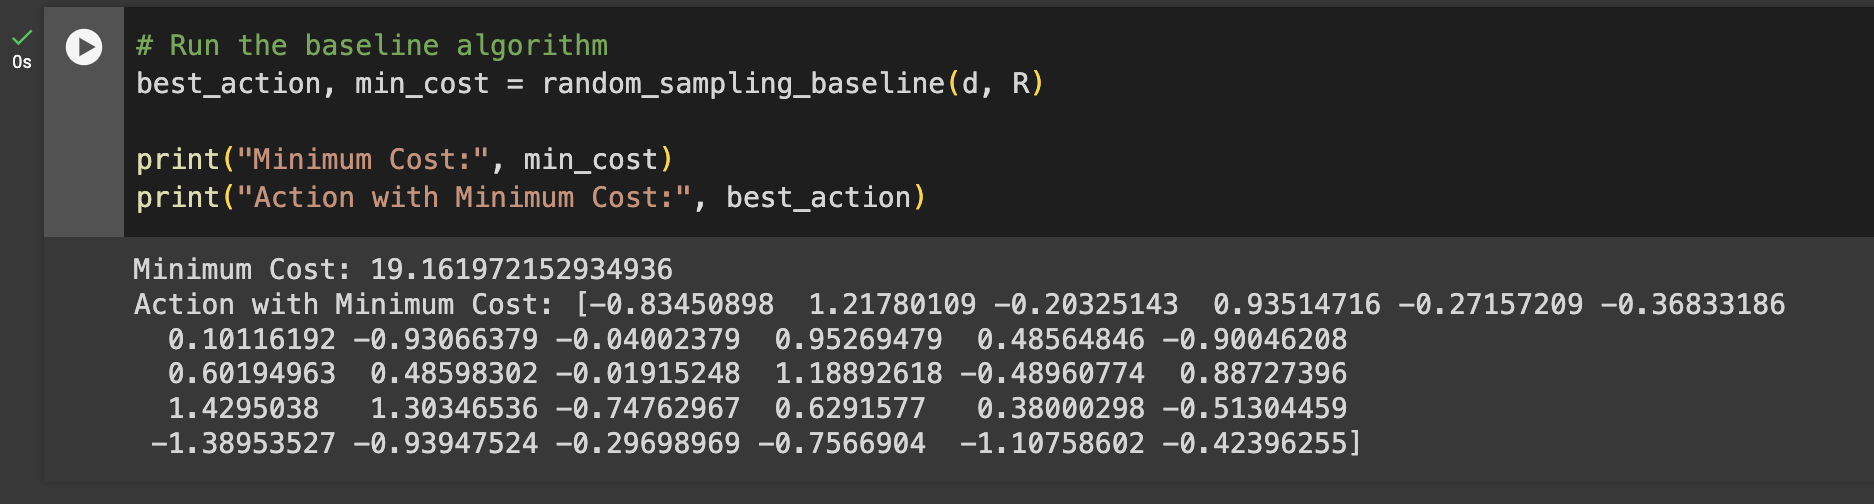
\includegraphics[scale=0.5]{BI.png}
    \item \underline{$R= $ random matrix}\par
    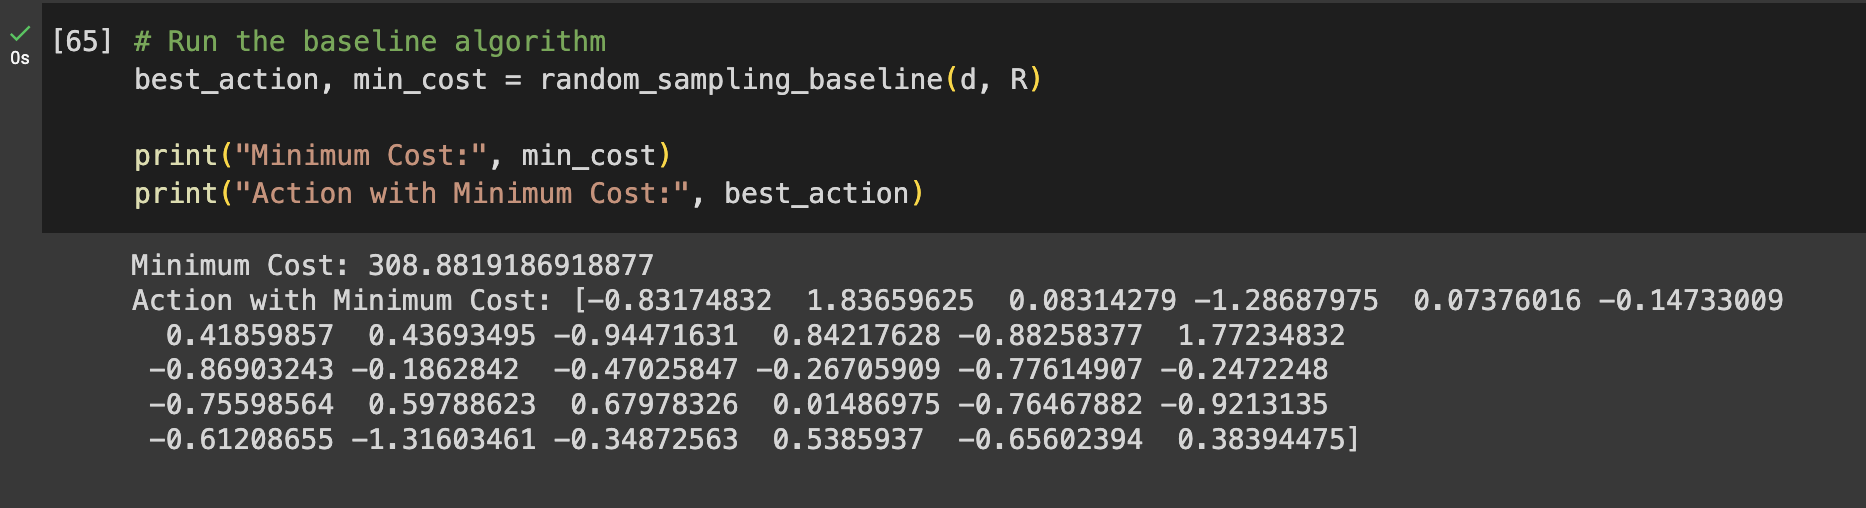
\includegraphics[scale=0.5]{BR.png}
\end{itemize}

\subsubsection*{Neural Network Algorithm}
Hyperparameters: 
\begin{verbatim}
    num_initial_samples = 500
    num_iterations = 95
    num_samples_per_iter = 100
    Total number of samples = 500 + (95 * 100) = 10,000
    learning_rate = 0.01
\end{verbatim}
\begin{itemize}
    \item \underline{$R = \mathbb{I}_{30}$}\par
    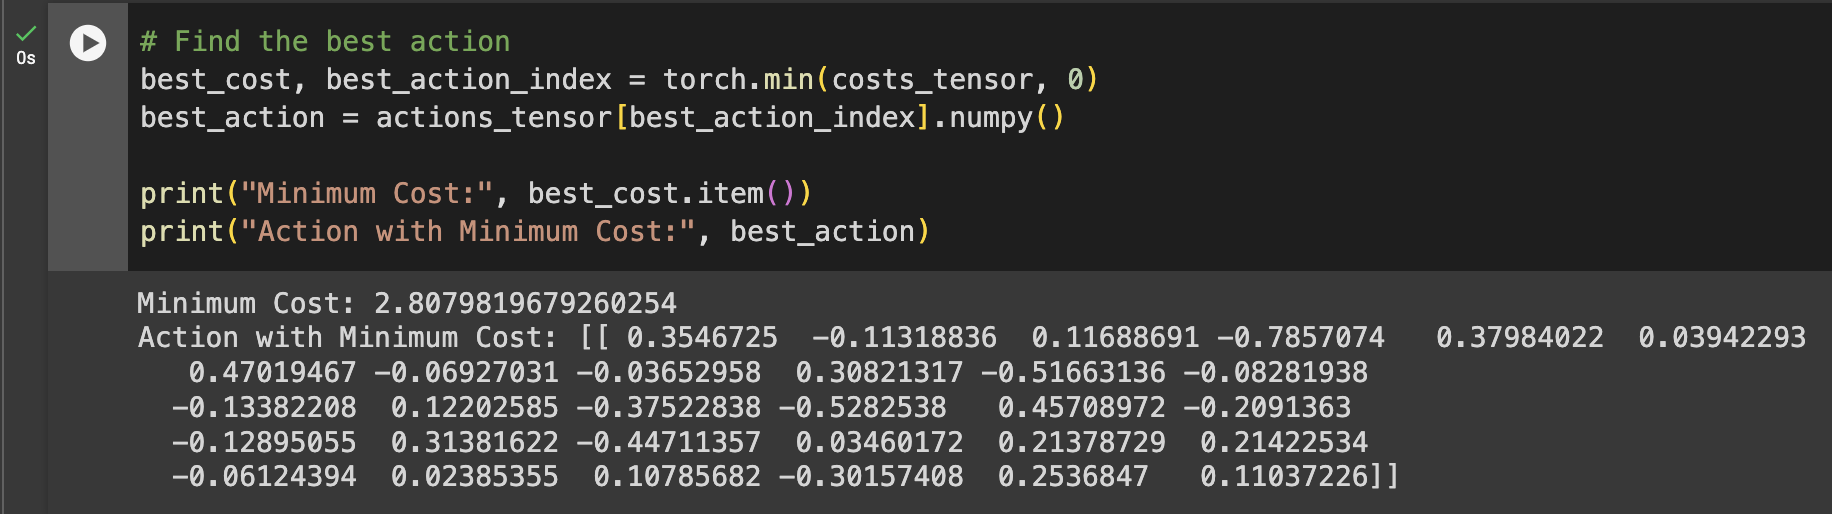
\includegraphics[scale = 0.5]{NI.png}
    \item \underline{$R= $ random matrix}\par
    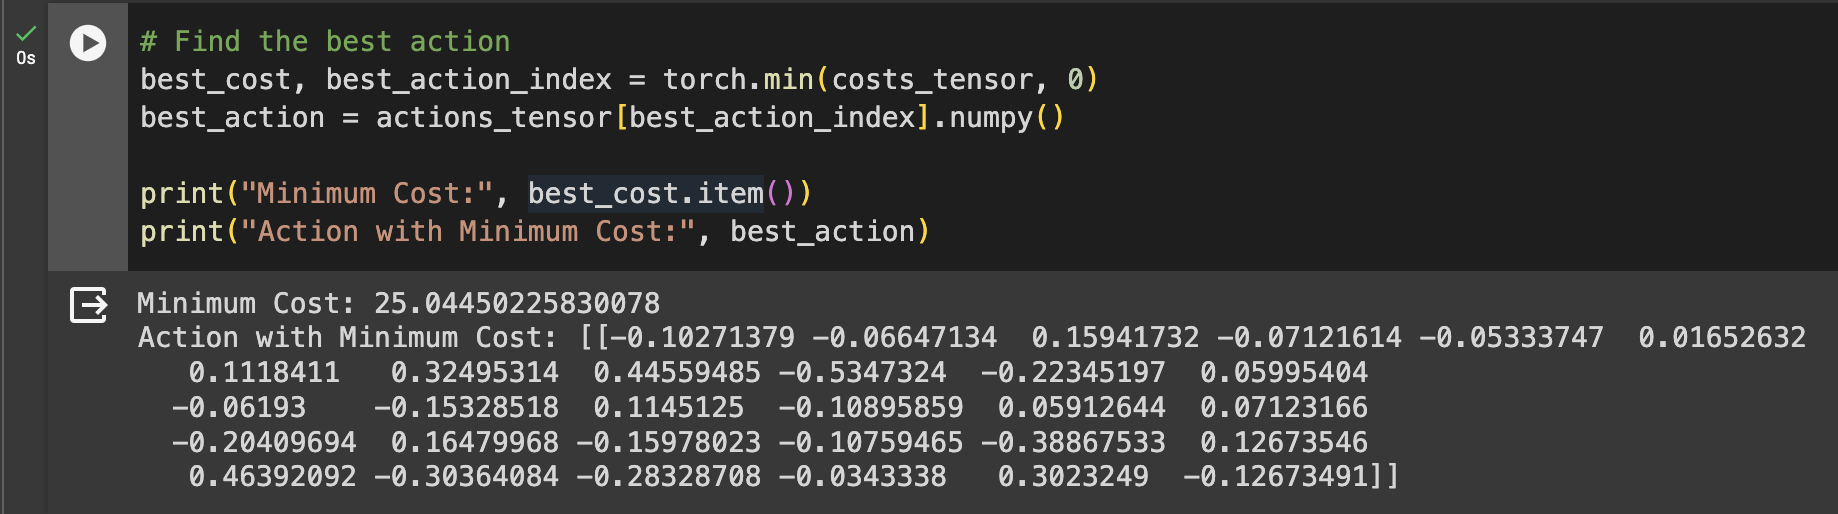
\includegraphics[scale=0.5]{NR.png}
\end{itemize}
%==================================================================================================
\section*{Part 2: Theory}
\begin{enumerate}[a)]
    \item \begin{proof}
        \renewcommand{\qedsymbol}{$\blacksquare$}
        \hfill\\\\
        \begin{equation*}
            \begin{aligned}
                P(\text{greedy action}) &= 1 - P(\text{not greedy action})\\
                &= 1 - P(\text{not greedy selection \textit{AND} not greedy action})\\
                &= 1 - P(\text{not greedy selection}) \cdot P(\text{not greedy action $|$ not greedy selection})\\
                &= 1 - \epsilon \cdot \left(\ddfrac{k-1}{k}\right) \textit{\hspace{1cm}$^{*}$ Since there is only \textbf{one} greedy action}\\
                &= 1 - \epsilon \cdot \left(1-\ddfrac{1}{k}\right)\\
                &= 1 - \epsilon + \ddfrac{\epsilon}{k}\\
            \end{aligned}
        \end{equation*}
    \end{proof}
    %==============================================
    \item  
    \begin{enumerate}[i)]
        \item \begin{proof}
            \renewcommand{\qedsymbol}{$\blacksquare$}
            \hfill\\\\
            To determine the probability that the greedy action was chosen for the first time at time $T$, we need to consider that it was not chosen at any time before $T$, and that it was chosen at time $T$.\\
            Thus, the following equation should be quantified:
            \begin{equation*}
                P(\text{greedy at } T) = P(\text{not greedy before } T) \cdot P(\text{greedy at } T)
            \end{equation*}
            Therefore, the probability that the greedy action was chosen for the first time at time $T$ is:
            \begin{equation*}
                \begin{aligned}
                    P(\text{greedy at } T) &= P(\text{not greedy before } T) \cdot P(\text{greedy at } T)\\
                    &= \left(1 - 1 + \epsilon - \frac{\epsilon}{k}\right)^{T - 1} \cdot \left(1 - \epsilon + \frac{\epsilon}{k}\right)\\
                    &= \left(\epsilon - \frac{\epsilon}{k}\right)^{T - 1} \cdot \left(1 - \epsilon + \frac{\epsilon}{k}\right)\\
                \end{aligned}
            \end{equation*}\par
        \end{proof}

    \item \begin{proof}
        \renewcommand{\qedsymbol}{$\blacksquare$}
        \hfill\\\\
        To get the expected number of steps, $\mathbb{E}[T]$, until the the greedy action is chosen for the first time is a sum over all possible time steps, each weighted by its probability of being the first time the greedy action is chosen.\\
        Thus, the following equation should be quantified:
        \begin{equation*}
            \mathbb{E}[T] = \sum_{t = 1}^{\infty} t \cdot P(\text{greedy at } t)
        \end{equation*}
        Following, the equation is 
        \begin{equation*}
            \begin{aligned}
                \mathbb{E}[T] &= \sum_{t = 1}^{\infty} t \cdot P(\text{greedy at } t)\\
                &= \sum_{t = 1}^{\infty} t \cdot \left(\epsilon - \frac{\epsilon}{k}\right)^{t - 1} \cdot \left(1 - \epsilon + \frac{\epsilon}{k}\right)\\
            \end{aligned}
        \end{equation*}
        It can be observed that the above equation is a geometric series, which can be simplified to the following:
        \begin{equation*}
            \begin{aligned}
                \mathbb{E}[T] &= \sum_{t = 1}^{\infty} t \cdot \left(\epsilon - \frac{\epsilon}{k}\right)^{t - 1} \cdot \left(1 - \epsilon + \frac{\epsilon}{k}\right)\\
                &= \ddfrac{1}{\left(\epsilon - \frac{\epsilon}{k}\right)^{t - 1} \cdot \left(1 - \epsilon + \frac{\epsilon}{k}\right)}
            \end{aligned}
        \end{equation*}\par
        The above simplifciation is valid due to the definiton of the expected value of a geometric series.\par 
    \end{proof}
    \end{enumerate}
    %==============================================
    \item 
    \begin{enumerate}[i)]
        \item 
        \begin{proof}
            \renewcommand{\qedsymbol}{$\blacksquare$}
            \hfill\\\\
            Firstly, denote $\max(q(1), q(2), \dots, q(10))$ as $q_{*}$.\\
            The algorithm will choose the greedy selection, $q_{*}$ with probability $1 - \epsilon$, and a non-greedy selection with probability $\epsilon$.\\
            Moreover, the expected value of the an action during non-greedy selection is the average of all the action values, which is $\frac{\sum_{i = 1}^{10} q(i)}{10}$.\\
            Therefore, the long-run reward is 
            \begin{equation*}
                R = (1 - \epsilon) \cdot q_{*} + \epsilon \cdot \frac{\sum_{i = 1}^{10} q(i)}{10}
            \end{equation*}\par 
        \end{proof}
        
        \item 
        \begin{proof}
           \renewcommand{\qedsymbol}{$\blacksquare$}
            \hfill\\\\
           Since $q(1), q(2), \dots, q(10)$ are i.i.d. random variables, the expected value of a greedy action becomes $\mathbb{E}[q_{*}] = b$.\\
           Moreover, since $q(a)$ is $\mathcal{N}(0,1)$, the expected average of all the action values becomes $\mathbb{E}\left[\frac{\sum_{i = 1}^{10} q(i)}{10}\right] = 0$.\\
           Therefore, the long-run reward is
           \begin{equation*}
               \begin{aligned}
                   R &= (1 - \epsilon) \cdot \mathbb{E}[q_{*}] + \epsilon \cdot \mathbb{E}\left[\frac{\sum_{i = 1}^{10} q(i)}{10}\right]\\
                   &= (1 - \epsilon) \cdot b + \epsilon \cdot 0\\
                   &= (1 - \epsilon) \cdot b
               \end{aligned}
           \end{equation*}\par 
        \end{proof}
    \end{enumerate}
    %==============================================
    \item 
    \begin{itemize}
        \item \underline{Restatement}
        In any stochastic bandit problem, denoted as \(\nu\), where you have a set of actions \(A\) that is either finite or can be counted (like a list), and a fixed number of rounds or steps \(n \in \mathbb{N}\), the regret \(R_n\) of following a certain strategy or policy \(\pi\) in this environment can be calculated as follows:
        \\\\
        The total regret \(R_n\) is the sum of the regrets for each individual action in \(A\). The regret for each action \(a\) is the product of two things: the suboptimality gap \(\Delta_a\) of action \(a\) (which is how much less reward you expect from action \(a\) compared to the best possible action), and the expected number of times \(E[T_a(n)]\) that action \(a\) is chosen within the first \(n\) rounds.

        Mathematically, this is represented as:
        \[ R_n = \sum_{a \in A} \Delta_a E[T_a(n)] \]
        This means you add up the products of the suboptimality gap and the expected number of selections for each action to find the total regret.

        \item \underline{Proof}
        \begin{proof}
            \renewcommand{\qedsymbol}{$\blacksquare$}
            \hfill\\\\
            Before the proof, we need to redefine the above terms to be consistent with S\&B's notation.\\
            Firstly, the set of actions, $A$, is the set of arms, $k$.\\
            Secondly, the suboptimality gap, $\Delta_a$, is the difference between the expected reward of the optimal action, $\underset{1\leq a \leq k}{\max} q_{*}(a)$, and the expected reward of action $q_{*}(a)$: 
            \begin{equation*}
                \Delta_a = \underset{1\leq a \leq k}{\max} q_{*}(a) - q_{*}(a)
            \end{equation*}
            Thirdly, the expected number of times $E[T_a(n)]$ that action $a$ is chosen within the first $n$ rounds is the expected number of times that action $a$ is chosen within the first $n$ rounds:
            \begin{equation*}
                \mathbb{E}[T_a(n)] = \mathbb{E}[N_{n}(a)]
            \end{equation*}\par 
            Since the regret is the difference in choosing the optimal action and the action chosen, it can be expressed as follows:
            \begin{equation*}
                \text{Reg}_{n} = n \cdot \underset{1\leq a \leq k}{\max} q_{*}(a) - \mathbb{E}[R_{n}]
            \end{equation*}
            where $n$ is the number of rounds, $\underset{1\leq a \leq k}{\max} q_{*}(a)$ is the expected reward of the optimal action, and $\mathbb{E}[R_{n}]$ is the expected reward of the action chosen up to round $n$.\\
            To further break down the term $\mathbb{E}[R_{n}]$, we can transform it into a term that descirbes actions, rather than rewards.\\
            Thus, consider the following representation:
            \begin{equation*}
                R_{n} = \sum_{t=1}^{n}\sum_{a = 1}^{k} R_{t}(a) \cdot \mathbbm{1}_{A_{t} = a}
            \end{equation*}
            Now, the regret can be expressed as follows:
            \begin{equation*}
                \begin{aligned}
                    \text{Reg}_{n} &= n \cdot \underset{1\leq a \leq k}{\max} q_{*}(a) - \mathbb{E}[R_{n}]\\
                    &= n \cdot \underset{1\leq a \leq k}{\max} q_{*}(a) - \mathbb{E}\left[\sum_{t=1}^{n}\sum_{a = 1}^{k} R_{t}(a) \cdot \mathbbm{1}_{A_{t} = a}\right]
                \end{aligned}
            \end{equation*}
            Using properties of the expected value and that we are summing over $n$ time steps, the above equation can be simplified to the following:
            \begin{equation*}
                \begin{aligned}
                    \text{Reg}_{n} &= n \cdot \underset{1\leq a \leq k}{\max} q_{*}(a) - \mathbb{E}\left[\sum_{t=1}^{n}\sum_{a = 1}^{k} R_{t}(a) \cdot \mathbbm{1}_{A_{t} = a}\right]\\
                    &= \sum_{a=1}^{k}\sum_{t=1}^{n} \mathbb{E}\left[\underset{1\leq a \leq k}{\max} q_{*}(a)-R_{t}(a) \cdot \mathbbm{1}_{A_{t}=a}\right]
                \end{aligned}
            \end{equation*}
            The expected reward on round $t$ is conditional on the action chosen on round $t$, $A_{t}$.\\
            Thus, the expected value term can be expressed as follows:
            \begin{equation*}
                \begin{aligned}
                    \mathbb{E}\left[\underset{1\leq a \leq k}{\max} q_{*}(a)-R_{t}(a) \cdot \mathbbm{1}_{A_{t}=a} | A_{t}\right] &= \mathbbm{1}_{A_{t}=a} \mathbb{E}\left[\underset{1\leq a \leq k}{\max} q_{*}(a)-R_{t}(a) | A_{t}\right]\\
                    &= \mathbbm{1}_{A_{t}=a} \left(\underset{1\leq a \leq k}{\max} q_{*}(a)-q(a)\right)\\
                    &= \mathbbm{1}_{A_{t}=a} \cdot \Delta_{a}\\
                \end{aligned}
            \end{equation*}
            The term $\sum_{t=1}^{n} \mathbbm{1}_{A_{t}=a}$ is the number of times that action $a$ is chosen within the first $n$ rounds, $N_{n}(a)$.\\
            Therefore, we get the final result that the formula for the regret is
            \begin{equation*}
                \text{Reg}_{n} = \sum_{a=1}^{k} \Delta_{a} \cdot \mathbb{E}[N_{n}(a)]
            \end{equation*}
        \end{proof}
    \end{itemize}

    \item  
    \begin{itemize}
        \item \underline{Algorithm Restatement in S\&B Terms}\par 
        \begin{enumerate}
            \item \textbf{Initialization:}
            \begin{itemize}
                \item For each action \( a \) (in \( 1, 2, ..., k \)):
                \begin{itemize}
                    \item Initialize action-value estimate \( Q_t(a) = 0 \).
                    \item Initialize the number of times action \( a \) has been chosen, \( N_t(a) = 0 \).
                \end{itemize}
            \end{itemize}
        
            \item \textbf{Loop for each step \( t = 1, 2, 3, ... \):}
            \begin{itemize}
                \item Select action \( A_t \) using the UCB criterion:
                \[ A_t = \underset{a}{\arg\max} \left[ Q_t(a) + c \sqrt{\frac{\ln t}{N_t(a)}} \right] \]
                where \( c \) is a confidence level parameter.
                
                \item Take action \( A_t \), observe reward \( R_t \).
                
                \item Update the action-value estimate for \( A_t \):
                \[ Q_{t+1}(A_t) = Q_t(A_t) + \frac{1}{N_t(A_t)} (R_t - Q_t(A_t)) \]
                
                \item Increment \( N_t(A_t) \).
            \end{itemize}
        \end{enumerate}

        \item \underline{Proof Restatement}\par 
        In a k-armed bandit problem using the UCB algorithm, for any time step \( t \), the expected regret \( R_t \) is bounded by:
\[ R_t \leq 3 \sum_{i=1}^{k} \Delta_i + \sum_{i: \Delta_i > 0} \frac{16 \log(t)}{\Delta_i} \]
where \( \Delta_i = q_*(a^*) - q_*(a_i) \) is the regret associated with choosing action \( a_i \) instead of the optimal action \( a^* \).


\begin{enumerate}
    \item \textbf{Optimal Action Assumption:}\par 
    Assume that the first arm \( a_1 \) is optimal, so \( q_*(a_1) = q_*(a^*) \), where \( q_*(a) \) represents the true value of action \( a \).\par

    \item \textbf{Regret Decomposition:}\par 
    The total regret after \( t \) steps is:
    \[ R_t = \sum_{i=1}^{k} \Delta_i E[N_t(a_i)] \]
    where \( E[N_t(a_i)] \) is the expected number of selections of action \( a_i \) up to time \( t \).\par

    \item \textbf{Defining "Good" Event \( G_i \):}\par 
    Define the good event \( G_i \) for a suboptimal arm \( a_i \) as:
    \[ G_i = \left\{ q_*(a_1) < \min_{\tau \leq t} UCB(a_1, \tau) \right\} \cap \left\{ \hat{q}_\tau(a_i) + \sqrt{\frac{2 \log(1/\delta)}{N_\tau(a_i)}} < q_*(a_1) \, \forall \, \tau \leq t \right\} \]
    where \( \hat{q}_\tau(a_i) \) is the estimated value of action \( a_i \) at time \( \tau \), \( N_\tau(a_i) \) is the number of times action \( a_i \) has been selected up to time \( \tau \), and \( \delta \) is a confidence level parameter.\par

    \item \textbf{Bounding \( E[N_t(a_i)] \) under \( G_i \):}\par 
    Show that under \( G_i \), \( a_i \) is selected at most \( u_i \) times, where \( u_i \) is a function of \( \Delta_i \) and \( \delta \). This leads to:
    \[ E[N_t(a_i)|G_i] \leq u_i \]\par

    \item \textbf{Bounding Probability of \( G^c_i \):}\par 
    The probability of the complement event \( G^c_i \) (where the good event does not occur) is small. It is bounded using concentration inequalities.\par

    \item \textbf{Expected Selection Bound:}\par 
    Combine these results to express \( E[N_t(a_i)] \):
    \[ E[N_t(a_i)] = E[N_t(a_i)|G_i]P(G_i) + E[N_t(a_i)|G^c_i]P(G^c_i) \leq u_i + t P(G^c_i) \]\par

    \item \textbf{Choosing \( u_i \) and \( c \):}\par 
    The choice of \( u_i \) is made to ensure that the upper confidence bound for suboptimal arm \( a_i \) is properly controlled. A natural choice for \( u_i \), considering the balance between exploration and exploitation, is given by:
    \[ u_i = \left\lceil \frac{2 \log(1/\delta)}{(1 - c)^2 \Delta_i^2} \right\rceil \]
    where \( \delta \) is the confidence level parameter, and \( c \) is a constant. 

    In the proof, \( c \) is chosen to be \( 1/2 \) somewhat arbitrarily but in a way that balances the two terms in the regret bound. This choice leads to a simplification of the regret bound while maintaining a balance between exploration and exploitation.

    \item \textbf{Finalizing the Bound on \( R_t \):}\par 
    With \( u_i \) and \( c \) chosen, the final bound on \( R_t \) is derived by substituting these values into the regret decomposition:
    \[ R_t \leq \sum_{i: \Delta_i > 0} \Delta_i \left( \left\lceil \frac{2 \log(1/\delta)}{(1 - c)^2 \Delta_i^2} \right\rceil + t P(G^c_i) \right) \]
    Applying the choice of \( c = 1/2 \), the final bound simplifies to:
    \[ R_t \leq 3 \sum_{i=1}^{k} \Delta_i + \sum_{i: \Delta_i > 0} \frac{16 \log(t)}{\Delta_i} \]
\end{enumerate}

        
        
    \end{itemize}
    
    \item 
    We consider a stochastic k-armed bandit problem where the goal is to maximize cumulative rewards over time.\\ 
    We use the Upper Confidence Bound (UCB) algorithm for arm selection. Let $Q_n$ be the average reward at time $n$ for a chosen arm, and let $a^*$ be the optimal arm.\\ 
    We aim to prove that:
    \[ \lim_{n \to \infty} \mathbb{E}[Q_n] = q_{*}(a^*) \]
    where $q_{*}(a^*)$ is the expected reward of the optimal arm.

    \begin{proof}
        \renewcommand{\qedsymbol}{$\blacksquare$}
        \hfill\\\\
        \begin{itemize}
            \item \underline{Theorem $7.1$ Condition}\par
            Theorem $7.1$ provides an upper bound on the regret $R_n$ for the UCB algorithm:
            Under the conditions of Theorem 7.1 and using Algorithm 3, the expected estimated value of the action selected at a large time step $n$ converges to the true value of the best action.

            \item \underline{Definition of $Q_n$}\par 
            $Q_n$ is defined as the average of rewards received from taking action $a$ up to time $t$:
            \[ Q_n = \frac{\sum_{i=1}^{t} R_i \cdot \mathbbm{1}_{A_i=a}}{\sum_{i=1}^{t} \mathbbm{1}_{A_i=a}} \]
            where $R_i$ is the reward received at time $i$, $A_i$ is the action taken at time $i$, and $\mathbbm{1}_{A_i=a}$ is the indicator function.
        \end{itemize}

        By the law of large numbers, for each arm $a$, the average reward converges to the expected reward $q_{*}(a)$ as $n$ increases.\\

        Therefore,
        \[ \frac{\sum_{i=1}^{n} R_i \cdot \mathbbm{1}_{A_i=a}}{\sum_{i=1}^{n} \mathbbm{1}_{A_i=a}} \to q_{*}(a) \]
        as $n \to \infty$.
        
        The UCB algorithm selects arms based on the estimated reward and the uncertainty in that estimate. Over time, it favors arms with higher estimated rewards.
        

        For the optimal arm $a^*$, as $n \to \infty$, the UCB algorithm will increasingly favor this arm, assuming it correctly identifies it. Therefore, the frequency of selecting arm $a^*$, denoted by $N_{a^*}(n)$, will dominate over other arms, leading to:
        \[ \frac{N_{a^*}(n)}{n} \to 1 \]
        and for each suboptimal arm $a$,
        \[ \frac{N_a(n)}{n} \to 0 \]
        

        Given the dominance of the optimal arm in selections, the limit of the expected average reward $\mathbb{E}[Q_n]$ converges to the expected reward of the optimal arm:
        \[ \lim_{n \to \infty} \mathbb{E}[Q_n] = q_{*}(a^*) \]
        

        Under the UCB algorithm, the expected average reward for the arm selected by the algorithm converges to the expected reward of the optimal arm as the number of trials $n$ goes to infinity.\par 
    \end{proof}
    
\end{enumerate}
%==================================================================================================
\end{document}